\documentclass[tikz,border=5pt]{standalone}
\usepackage{fontspec}
\setmainfont{Times New Roman}
\usepackage{unicode-math}
\setmathfont{Cambria Math}
\usetikzlibrary{shapes.geometric,positioning,fit,backgrounds,arrows.meta,calc}

\begin{document}
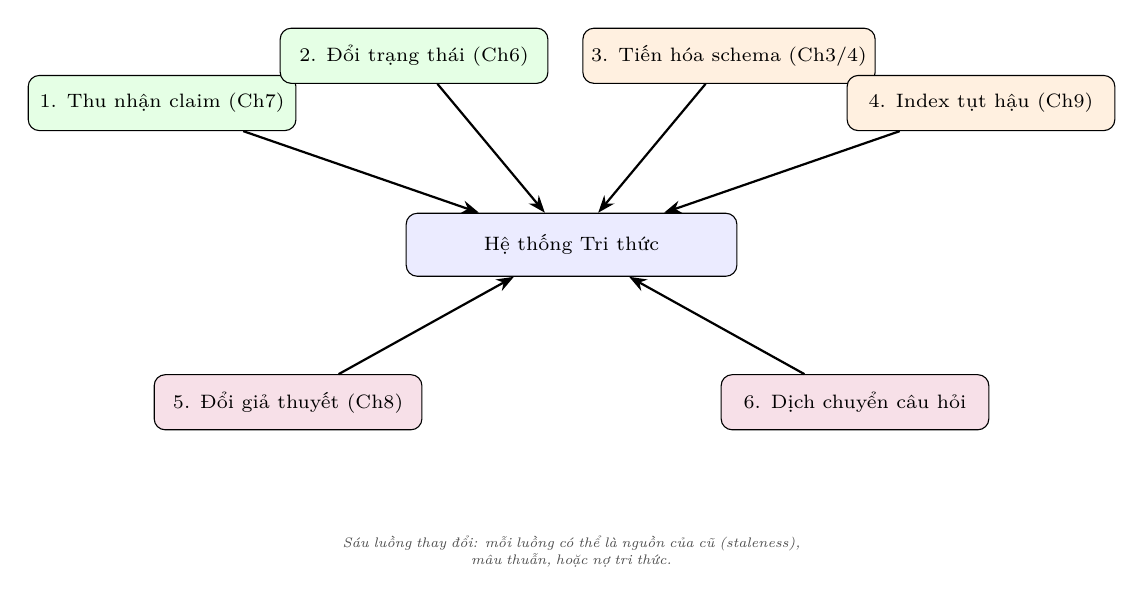
\begin{tikzpicture}[
  box/.style={rectangle, draw, rounded corners, align=center, font=\scriptsize, inner sep=3pt},
  arrow/.style={-{Stealth[length=2.2mm]}, thick},
  label/.style={font=\tiny\itshape, text=gray!60!black},
]

% === SIX FLOWS OF CHANGE ===
\node[box, fill=blue!8, minimum width=4.2cm, minimum height=0.8cm] (sys) at (0, 2.6) {Hệ thống Tri thức};

\node[box, fill=green!10, minimum width=3.4cm, minimum height=0.7cm] (f1) at (-5.2, 4.4) {1. Thu nhận claim (Ch7)};
\node[box, fill=green!10, minimum width=3.4cm, minimum height=0.7cm] (f2) at (-2.0, 5.0) {2. Đổi trạng thái (Ch6)};
\node[box, fill=orange!12, minimum width=3.4cm, minimum height=0.7cm] (f3) at (2.0, 5.0) {3. Tiến hóa schema (Ch3/4)};
\node[box, fill=orange!12, minimum width=3.4cm, minimum height=0.7cm] (f4) at (5.2, 4.4) {4. Index tụt hậu (Ch9)};
\node[box, fill=purple!12, minimum width=3.4cm, minimum height=0.7cm] (f5) at (-3.6, 0.6) {5. Đổi giả thuyết (Ch8)};
\node[box, fill=purple!12, minimum width=3.4cm, minimum height=0.7cm] (f6) at (3.6, 0.6) {6. Dịch chuyển câu hỏi};

\draw[arrow] (f1) -- (sys);
\draw[arrow] (f2) -- (sys);
\draw[arrow] (f3) -- (sys);
\draw[arrow] (f4) -- (sys);
\draw[arrow] (f5) -- (sys);
\draw[arrow] (f6) -- (sys);

\node[label, align=center, text width=11cm] at (0, -1.3)
  {Sáu luồng thay đổi: mỗi luồng có thể là nguồn của cũ (staleness),\\mâu thuẫn, hoặc nợ tri thức.};
\end{tikzpicture}
\end{document}